\subsection{Cracking Minesweeper: Donald Knuth's version}

\renewcommand{\CURPATH}{equations/minesweeper_Knuth}

From Donald Knuth's TAOCP Section 7.2.2.2:

\begin{figure}[H]
\centering
\frame{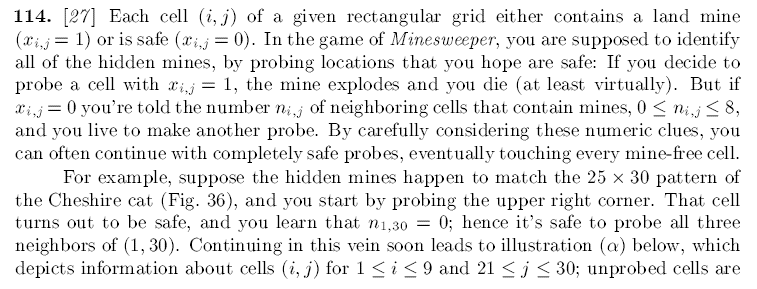
\includegraphics[scale=0.85]{\CURPATH/minesweeper1.png}}
\end{figure}

\begin{figure}[H]
\centering
\frame{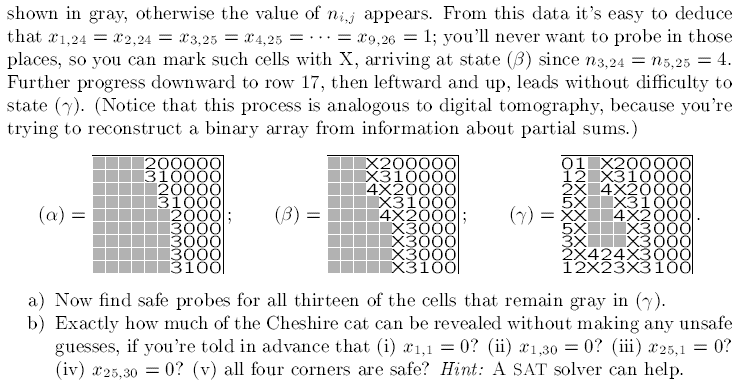
\includegraphics[scale=0.85]{\CURPATH/minesweeper2.png}}
\end{figure}

And solution:

\begin{figure}[H]
\centering
\frame{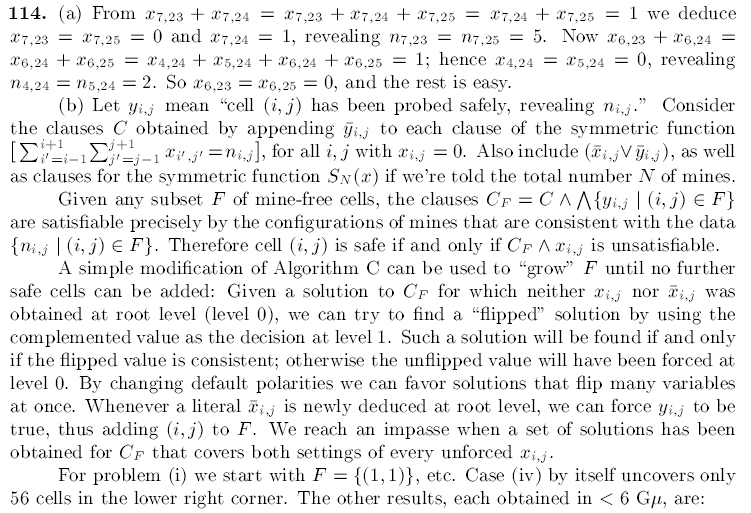
\includegraphics[scale=0.85]{\CURPATH/minesweeper3.png}}
\end{figure}

\begin{figure}[H]
\centering
\frame{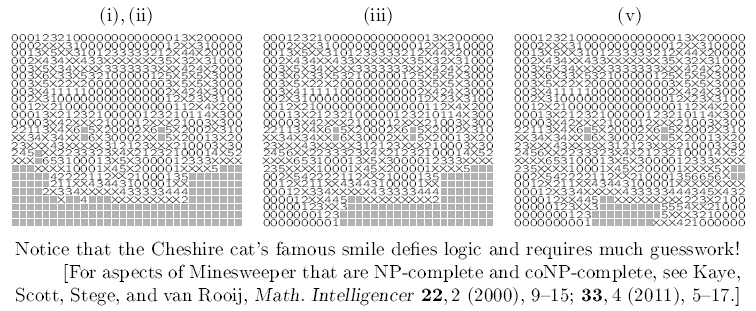
\includegraphics[scale=0.85]{\CURPATH/minesweeper4.png}}
\end{figure}
